\documentclass[11pt,a4paper]{article}
\usepackage{fontspec}
\setmainfont{Source Serif 4}[Path=/home/claude/ref/fonts/, UprightFont=SourceSerif4-Regular.ttf, BoldFont=SourceSerif4-Semibold.ttf, ItalicFont=SourceSerif4-It.ttf]
\setmonofont{IBM Plex Mono}[Path=/home/claude/ref/fonts/, UprightFont=IBMPlexMono-Regular.ttf, BoldFont=IBMPlexMono-Medium.ttf, Scale=0.88]
\usepackage[margin=2.5cm]{geometry}
\usepackage{graphicx,booktabs,longtable,array,caption,amsmath,xcolor,setspace}
\usepackage[authoryear,round]{natbib}
\usepackage[hidelinks]{hyperref}
\usepackage{microtype}
\setstretch{1.12}
\captionsetup{font=small,labelfont=bf}
\setlength{\bibsep}{3pt}
\title{\textbf{Who Gets Talked About? Public Attention on Wikipedia and Parliamentary Attention in the House of Commons to UK Places, 2005 to 2025}}
\author{Tristan Hotham\\\small Independent researcher\\\small ORCID 0000-0003-4931-9349}
\date{2026}
\begin{document}
\maketitle
\begin{center}\textbf{Abstract}\end{center}
Which places does Parliament talk about, and how closely does that follow what the public is interested in? I link counts of House of Commons contributions that mention UK towns and cities (``in'' plus the place name, 2005 to 2025) to the English Wikipedia pageviews of the same places in 2024, for 1,425 matched places. The two kinds of attention are strongly related (Spearman $\rho$ = 0.74). In a pre-specified Poisson model with population, region, distance from London and deprivation, the elasticity of mentions with respect to pageviews is 0.54 (95\% CI 0.46 to 0.62). The clearest departure from public attention is representational: places whose name forms part of a Commons constituency name are mentioned 121\% more often (95\% CI 90 to 158), a pattern that random reassignment does not reproduce and phrase matching does not explain away; within places, gaining a seat name at a boundary change is followed by more mentions, but leads show a pre-existing upward trend, so the within-place estimate probably overstates any effect of the name. There is no evidence of a deficit for places in the devolved nations: Welsh places receive 64\% more mentions than English places with the same attention (CI 38 to 96), robust to every check, while apparent north/south contrasts depend on London alone. The link between the two attentions weakened between 2005 to 2014 and 2015 to 2025. The design is correlational and pageviews are a noisy measure of public interest; the contribution is a transparent, reusable place-level comparison of the two attentions.

\medskip\noindent\textbf{Keywords:} political attention; parliamentary debate; Hansard; Wikipedia pageviews; constituency representation; geography of representation; United Kingdom

\section{Introduction}
Parliaments talk about places. Members of the House of Commons are elected for territorial constituencies, raise the problems of named towns, and argue over where money, hospitals and railways should go. The public, too, pays attention to places, for reasons that overlap only partly with politics: people look up where they live, where they might move, where they will go on holiday, and where something happened in the news. A long tradition in political science studies how far the attention of governments and legislatures follows public priorities \citep{BaumgartnerJones1993,JonesBaumgartner2005,JenningsJohn2009,BevanJennings2014}. Another studies how legislators represent territory, through constituency service, questions and speeches \citep{CainFerejohnFiorina1987,NortonWood1993,Searing1994,Martin2011,Russo2011,Kellermann2016,Zittel2019}. A third, newer literature, written mostly in the aftermath of the 2016 referendum, argues that some places feel unheard: ``places that don't matter'' \citep{RodriguezPose2018}, ``left behind'' towns \citep{JenningsStoker2016,McCann2020}, and rural communities that resent distant elites \citep{Cramer2016}.

These literatures share a question they rarely measure directly at the level of the place: which places get talked about in Parliament, relative to what we would expect from their size and from the public's own interest in them? This paper answers that question for the United Kingdom. I set two place-level measures side by side. Parliamentary attention is the number of House of Commons contributions from 2005 to 2025 that contain the phrase ``in'' followed by the place name, taken from an existing open count of Hansard \citep{Hotham2026}. Public attention is the number of times readers opened the English Wikipedia article on the place in 2024. Wikipedia pageviews have been used as a measure of collective attention in studies of film audiences, elections, markets, disease and memory \citep{Mestyan2013,YasseriBright2016,Moat2013,Generous2014,GarciaGavilanes2017}; here they serve as a broad, public, freely available indicator of how much interest a place attracts.

The paper makes four contributions. First, it builds a documented link between 1,661 Hansard place terms and Wikipedia articles through Wikidata, with explicit rules for ambiguous names, name collisions and renamed articles, and reports the match rate (98.4\%) and every exclusion. Second, it estimates how strongly parliamentary attention follows public attention once population is held constant, and where the two diverge. Third, it tests a representational mechanism: whether places that give their name to a constituency receive more parliamentary attention than equally prominent places that do not, using both cross-sectional comparisons and the boundary changes of 2010 and 2024. Fourth, it tests whether the geography of parliamentary attention shows a deficit for the devolved nations or for the North of England once public attention is held constant. The analysis plan, hypotheses and robustness checks were written down before any outcome model was run, and the planned specification is reported as the main result.

The answers are mixed in instructive ways. The two attentions agree broadly, but parliamentary mentions rise less than proportionally with public interest. Having a seat named after a place is the strongest predictor of parliamentary attention beyond size and interest, although the within-place evidence shows that places which gain seat names were already becoming more prominent. There is no sign of a devolved-nation deficit; Welsh places are, if anything, mentioned more. Apparent regional contrasts in England rest on a single observation, London. And the two kinds of attention drifted apart over the period. All of this is correlational, and Section~\ref{sec:discussion} sets out what the data cannot show.

\section{Background and literature}
\subsection{Political attention and its correspondence with public priorities}
The agenda-setting tradition treats attention as scarce: governments and legislatures cannot attend to everything, so what they choose to talk about reveals priorities and responsiveness \citep{BaumgartnerJones1993,JonesBaumgartner2005}. Studies of the United Kingdom have shown that executive agendas respond to public concerns about issues \citep{JenningsJohn2009} and that this responsiveness varies across venues and institutions \citep{BevanJennings2014}. Parliamentary questions and debates are among the most flexible of these venues, and their content responds to media and public agendas \citep{VliegenthartWalgrave2011}. The thermostatic model of opinion and policy \citep{SorokaWlezien2010} and the broader literature on representation \citep{Pitkin1967,EulauKarps1977,Mansbridge2003} supply the normative frame: a responsive legislature should in some sense attend to what the public cares about.

This literature almost always measures attention to \emph{issues}: health, crime, the economy. Attention to \emph{places} is less studied, although it is central to territorial representation. Debate in the Commons has long been studied through its text \citep{EggersSpirling2014,ProkschSlapin2015}, but rarely as a distribution of attention across the map. One recent open data study counted place mentions in Hansard from 1909 to 2025 and showed that mentions grow faster than population and that a few towns are mentioned far more than their size predicts \citep{Hotham2026}. That study had no measure of how much interest each place commands outside Parliament, which is the gap filled here.

\subsection{Territorial representation and the constituency link}
Members of single-member districts have incentives to cultivate a personal vote by serving and speaking for their constituency \citep{CainFerejohnFiorina1987}. British MPs spend substantial time on constituency work \citep{NortonWood1993,Searing1994}, and voters say they value it \citep{VivyanWagner2016}. Parliamentary questions have become the standard measure of constituency focus \citep{Martin2011,Russo2011,Zittel2019}, and in the Commons constituency-oriented activity responds to electoral vulnerability \citep{Kellermann2013,Kellermann2016}; private members' bills show a similar if weaker electoral connection \citep{Bowler2010}. Constituency focus also varies with the electoral calendar in party-constrained systems \citep{Fernandes2018}.

What this literature implies for places is direct. Constituencies are named after towns, cities and areas, and each MP has an obvious reason to name the places in their seat. A place that gives its name to a seat has, in effect, a designated spokesperson. A place absorbed into a seat named after somewhere else, or after a compass point and a county, may be mentioned less even if it is equally large and equally interesting to the public. This is the representational mechanism tested here. It is not a test of whether MPs serve their constituents well; it is a test of whether the naming of the electoral map shapes which places are spoken of.

\subsection{Places that feel unheard}
A large literature on the geography of discontent argues that economic decline and the concentration of growth in London and the South East have left many places, often in the North of England and in coastal and industrial towns, feeling ignored by Westminster \citep{RodriguezPose2018,McCann2020}. \citet{JenningsStoker2016} describe a bifurcation between cosmopolitan and backwater England; \citet{Cramer2016} documents how rural residents in Wisconsin interpret their place as overlooked by urban decision makers. Devolution adds a further layer: since 1999 many domestic matters in Scotland, Wales and Northern Ireland have been decided by devolved legislatures, and debates about English representation at Westminster have followed \citep{Kenny2014}. Two expectations follow for parliamentary attention to places. A ``voice deficit'' view predicts that northern and deprived places receive less attention than their prominence warrants. A ``problem attention'' view, closer to agenda-setting theory and to news values \citep{GaltungRuge1965}, predicts the opposite: legislatures talk about places when something is wrong there, so deprivation and decline attract mentions. For the devolved nations, the transfer of policy competence predicts fewer Commons mentions for their places, conditional on how much the public cares about them.

\subsection{Wikipedia pageviews as a measure of public attention}
Search and pageview data offer behavioural measures of attention that do not rely on surveys. Search queries tracked influenza \citep{Ginsberg2009}, and Google Trends has been used, with caveats about what it measures, as an indicator of issue salience \citep{Mellon2013}. Wikipedia pageviews are open, available per article and per day, and have been used to forecast box office takings \citep{Mestyan2013} and disease \citep{Generous2014}, to study markets \citep{Moat2013} and collective memory \citep{GarciaGavilanes2017}, to forecast tourism demand \citep{Khadivi2016}, and to study elections, where \citet{YasseriBright2016} caution that pageviews measure interest, not support, and need theoretically informed models. Surveys of readers show a mix of motives: looking up a fact, reading in depth, responding to the news or to media, and personal curiosity \citep{Singer2017,Lemmerich2019}. The geography of Wikipedia content is itself uneven \citep{Graham2014}. For this study the implication is that pageviews of a place's article capture a blend of residents' interest, tourism, news events and the place's general cultural prominence, read by a worldwide English-speaking audience. That blend is what I call public attention; the robustness checks probe its main distortions.

\subsection{Contribution}
To my knowledge, no study has compared the distribution of parliamentary attention across places with an independent behavioural measure of public attention to the same places. The contribution is fourfold: a documented and reusable linkage of Hansard place counts to Wikipedia; estimates of the place-level correspondence between the two attentions; a test of the constituency-naming mechanism with cross-sectional and within-place designs; and a test of regional and national deficits conditional on public attention.

\section{Data}
\subsection{Parliamentary attention}
Parliamentary attention comes from \emph{Mentioned in the House} \citep{Hotham2026}, which used the UK Parliament Hansard search to count, for each year from 1900 to 2026, House of Commons spoken contributions that contain the quoted phrase ``in'' followed by a place name, for 1,661 UK place terms. The ``in'' phrase is a sample of all mentions, but a deliberate one: it is not inflated by the formula ``the hon. Member for'', by surnames, or by division lists, all of which affect simple name counts. That source flagged names shared by two UK places (26), names with a better-known namesake such as Perth or Boston (29), and names that are ordinary words (Reading, Deal, March); for the latter it estimated the share of sampled contributions that referred to the place and scaled the counts, or left the name out when that share was below 60\%. Where one name begins with another (Bury and Bury St Edmunds) the longer name's counts were subtracted from the shorter one's. I use the scaled yearly counts and sum them over 2005 to 2025 (21 full years), and over the sub-periods 2005 to 2014 and 2015 to 2025. The same source also provides any-mention counts from 2005, used here only as a robustness outcome. The names of Commons seats in each boundary period are those contested at the 2005, 2010 and 2024 general elections (646, 650 and 650 seats), from an open dataset of UK general election contests \citep{Hotham2026b}.

\subsection{Public attention}
Public attention is the number of English Wikipedia pageviews by human readers (the ``user'' agent, excluding identified bots and spiders) of each place's article, summed over calendar year 2024, from the Wikimedia pageview API. Articles were identified from Wikidata \citep{Vrandecic2014}: all items that are instances of human settlements in the United Kingdom with an English Wikipedia article (29,913 items), with their population and coordinates. Pageviews were collected for the 5,191 articles of settlements with a recorded population of at least 1,500; 8 returned zero views and none failed. The Wikidata set includes 81 items outside the United Kingdom, among them Gibraltar and capitals of British Overseas Territories; all were removed by requiring that the point lie within (or within 3 km of) a UK local authority district.

\subsection{Linking the two}
Each Hansard term was matched to a Wikidata settlement whose article title, without any comma qualifier or bracketed qualifier (``Reading, Berkshire'' becomes ``Reading''), equals the term after normalising case, accents, apostrophes and hyphens, and treating ``Saint'' as ``St''. Short forms used in debate were linked to their full names (Hull to Kingston upon Hull, Southend to Southend-on-Sea). Candidates had to lie within 0.31 km of the Hansard point at the median and within 20 km at most; among several candidates, one with pageviews, then one without a bracketed qualifier, then the nearest was chosen. 16 spelling differences were resolved by hand (for example Y Bala to Bala, Gwynedd) and one name was dropped because in debate it means a London borough rather than the town (Barnet); all are listed in the replication files. Table~\ref{tab:flow} shows the result: 1,634 of 1,661 terms (98.4\%) were matched, and 1,503 (90.5\%) to an article with 2024 pageviews; the others mostly lack a Wikidata population of 1,500 or more, so their pageviews were not collected. Twenty-three terms had no Wikidata settlement of that name (Margate, Rhondda, Saddleworth and Hayling Island among them) and three had one only beyond 20 km. The full match list was read by eye.

Three further rules address ambiguity on the Wikipedia side. A Hansard ``in Ripley'' may refer to Ripley in Derbyshire or Ripley in Surrey; when another UK settlement of the same name had at least a quarter of the matched article's pageviews, the place was excluded as a name collision (20 places); a strict rule excluding any namesake with an article (53) is a robustness check. Three articles had implausibly few views for their population (below 2\% of it), most likely because the article was renamed during 2024 and its views split across titles; they were excluded. Two pairs of Hansard terms matched the same article (Newark and Newark-on-Trent; Dereham and East Dereham); because the longer name's counts had already been subtracted from the shorter one's, the two were added.

\subsection{Covariates}
Population is the 2021 Census built-up area population for England and Wales where the Hansard source had one (1,028 places) and the Wikidata population otherwise (397); Wikidata populations are of mixed vintages and definitions, so a Wikidata-only population and the exclusion of places where the two sources differ by more than a factor of three are robustness checks. Each place was located in a 2010 Westminster constituency (Great Britain), from which come its region (nine English regions, Scotland and Wales) and a deprivation measure from the 2011 Census: the percentage of households deprived in two or more of four dimensions (employment, education, health and housing), standardised. Northern Ireland places form a twelfth region and take the British mean for deprivation, so that their difference is absorbed by the region effect. Distance from London is the great-circle distance to Charing Cross. The seat-name share is the share of 2005 to 2025 (weighted by the three boundary periods: 2005 to 2010, 2010 to 2024 and from 2024) during which the place's name formed part of the name of a Commons seat, matched on whole words, with a name that sits inside a longer place name in the same seat not counted (``Bury'' in ``Bury St Edmunds''). Every match was checked against the distance between the place and the seat, and five whole-word matches that name a different place were removed (Colne in Colne Valley, Conwy in Meirionnydd Nant Conwy, Derby in Liverpool West Derby, Leigh in Southend West and Leigh, Sutton in Plymouth Sutton). 468 of the 1,425 places (33\%) were part of a seat name at some point. A disambiguated-title indicator marks articles whose title carries a qualifier, since readers who type the bare name may land on a disambiguation page or on another place, lowering views.

\subsection{The analysis sample}
The main sample contains the 1,425 places with a clean Hansard count, a matched article with positive 2024 pageviews, no name collision and a population (1,087 in England, 187 in Scotland, 137 in Wales and 14 in Northern Ireland; Table~\ref{tab:desc}). They account for 110,684 ``in'' mentions from 2005 to 2025 and 89,318,876 pageviews in 2024. The median place has 14,168 residents, 29,145 pageviews and 13 mentions; 81 places have none.

\begin{table}[tbp]\centering\small\caption{From Hansard place terms to the analysis sample.}\label{tab:flow}\begin{tabular}{lr}\toprule Step & Places\\\midrule
Hansard place terms (Mentioned in the House) & 1,661\\
\quad matched to a Wikidata settlement article & 1,634\\
\quad with 2024 pageviews collected & 1,503\\
\quad less: flagged in Hansard (shared, namesake, word) or merged duplicate & $-$55\\
\quad less: name collision with an equally viewed namesake & $-$20\\
\quad less: suspect (probably renamed) article & $-$2\\
\quad less: zero pageviews & $-$1\\\midrule
Main sample & 1,425\\\bottomrule\end{tabular}\end{table}
\begin{table}[tbp]\centering\small\caption{The main sample by nation: medians of population, 2024 pageviews and ``in'' mentions 2005 to 2025, total mentions, and the share of places that were part of a seat name.}\label{tab:desc}\begin{tabular}{lrrrrrr}\toprule Nation & $N$ & Population & Views & Mentions & Total mentions & Seat name (\%)\\\midrule
England & 1,087 & 16,115 & 30,726 & 13 & 93,519 & 37\\
Scotland & 187 & 8,830 & 24,930 & 8 & 9,389 & 21\\
Wales & 137 & 5,759 & 20,641 & 9 & 5,569 & 14\\
Northern Ireland & 14 & 29,190 & 65,258 & 40 & 2,207 & 21\\
\midrule
All & 1,425 & 14,168 & 29,145 & 13 & 110,684 & 33\\
\bottomrule\end{tabular}\end{table}

\section{Research design}
\label{sec:design}
The plan below was recorded in the project notes before any outcome model was estimated; the deviations are listed at the end of this section.

\paragraph{Hypotheses.} H1 (attention): conditional on population, places with more public attention receive more parliamentary attention. H2 (representation): places whose name forms part of a seat name receive more parliamentary attention than places with the same public attention and population. H3 (geography): (a) conditional on public attention and population, places in Scotland, Wales and Northern Ireland receive fewer Commons mentions than places in England; (b) within England, the voice-deficit view predicts fewer mentions for northern places (North East, North West, Yorkshire and the Humber) than for southern places (South East, South West, East of England), and the problem-attention view predicts more mentions for deprived places; H3b was stated as two-sided. H4 (stability): the places over- and under-mentioned relative to attention are stable between 2005 to 2014 and 2015 to 2025, judged by a Spearman correlation of at least 0.6 between the two periods' residuals. Evidence against H1 or H2 would be a 95\% interval including zero; against H3a, a devolved-nation contrast that includes zero or is positive.

\paragraph{Main specification (M1).} The outcome $Y_i$ is a count with many small values and a long right tail, so I estimate a Poisson pseudo-maximum-likelihood model \citep{SantosSilvaTenreyro2006}:
\begin{equation}
E[Y_i \mid X_i] = \exp\big(\beta_1 \log V_i + \beta_2 \log P_i + \beta_3 S_i + \beta_4 \log(1 + D_i) + \beta_5 Z_i + \beta_6 Q_i + \gamma_{r(i)}\big),
\end{equation}
where $V_i$ is 2024 pageviews, $P_i$ population, $S_i$ the seat-name share, $D_i$ distance from London in km, $Z_i$ standardised deprivation, $Q_i$ the disambiguated-title indicator and $\gamma_r$ region fixed effects (South East as reference). PPML is consistent under heteroskedasticity, handles zeros, and does not require the counts to be Poisson distributed. Standard errors are clustered by 2023 local authority district (353 clusters), because neighbouring places share MPs, local news and unmeasured shocks \citep{CameronMiller2015,Abadie2023}. Coefficients on logged variables are elasticities; for the seat share and contrasts I report $100(\exp(b)-1)$, the percentage difference in expected mentions. The region contrasts in H3 are population-weighted averages of region effects with cluster-robust standard errors from the full covariance matrix. Estimation used pyfixest and was checked against statsmodels.

\paragraph{Within-place design (M2).} Cross-sectional comparisons cannot separate the effect of a seat name from the reasons a place gets one. Seat names change at boundary reviews, which took effect in England, Wales and Northern Ireland in 2010 and across the United Kingdom in 2024. M2 is a PPML panel of yearly mentions for each place from 2005 to 2025 with place and year fixed effects \citep{Correia2020}, where the treatment is the share of the year during which the place's name was part of a seat name. 127 places changed status (21 gained a name at 2010 and 8 lost one; 87 gained and 13 lost at 2024).

\paragraph{Robustness (pre-specified).} (R1) Alternative specifications: OLS of $\log(1+Y)$; PPML with views and population only; no distance. (R2) Rank correlations, raw and partial on population. (R3) Outliers: dropping the top 1\% by views or by mentions, dropping London, dropping the London region. (R4) Leaving out one region at a time. (R5) Measurement: outcome restricted to 2024 (the year of the pageviews) or 2020 to 2025; any-mention outcome; Wikidata population only; dropping places whose population sources disagree; strict and permissive collision rules; dropping names scaled for word ambiguity; keeping suspect titles; exact titles only. (R6) Placebo and falsification: a permutation test reassigning seat-name shares at random within region by population-quintile cells (1,000 draws); a lead test in M2 adding the seat-name status two years ahead, whose coefficient should be near zero if mentions do not anticipate the change; and a fake-timing model with only the lead.

\paragraph{The over- and under-representation index.} For description and for the map, expected mentions come from a PPML of $Y_i$ on log views and log population only; the index is $(Y_i + 0.5)/(\hat Y_i + 0.5)$. Rankings include only places expected to receive at least 20 mentions.

\paragraph{Deviations from the plan.} Three changes were made after the plan was written, each before re-estimating and each reported. (i) The two pairs of duplicate Hansard terms were combined, a data correction found when reading the rankings. (ii) Reading the rankings also showed that long formal names (Saltburn-by-the-Sea, Newcastle upon Tyne, the City of London) are said in short forms in debate, so their ``in'' counts are artefacts; such names, and names never once found after ``in'' since 1909 or containing an apostrophe, are flagged (``name form'') and excluded from the rankings, and excluding them from the model is an added robustness check. The main model keeps them, as planned. (iii) The lead test failed (Section~\ref{sec:results}), so I added event-study models, labelled exploratory. An analysis of how 2024 pageviews relate to older debates is also exploratory. (iv) Two corrections were made at an independent review, before the final estimates: the seat names of each boundary period were taken from the complete lists of seats contested at the 2005, 2010 and 2024 elections, replacing a seat list built from members' histories that lacked some seats (for example Bath and Neath before 2015) and so recorded false changes of status, and five whole-word seat matches that name a different place were removed. The seat-name types analysis in Section~\ref{sec:results} was added at the same review and is exploratory.

\section{Results}
\label{sec:results}
\subsection{How closely the two attentions agree (H1)}
The rank correlation between 2024 pageviews and 2005 to 2025 mentions is 0.74, higher than between population and mentions (0.68); the partial rank correlation of views and mentions given population is 0.56 (Figure~\ref{fig:scatter}). In M1 (Table~\ref{tab:main}) the elasticity of mentions with respect to pageviews is 0.54 (95\% CI 0.46 to 0.62, $N$ = 1,425): doubling a place's pageviews at the same population is associated with 45\% more mentions (37 to 54\%). The population elasticity is 0.60 (0.52 to 0.68); the two together sum to more than one, consistent with the superlinear scaling of many urban quantities \citep{Bettencourt2007} and with the earlier finding that mentions grow faster than population \citep{Hotham2026}. Without views (M0), the population elasticity is 1.06. H1 is supported, with the qualification that parliamentary attention responds less than proportionally to public attention. The pseudo-$R^2$ of M1 is 0.94, dominated by the largest places.

\begin{figure}[tbp]\centering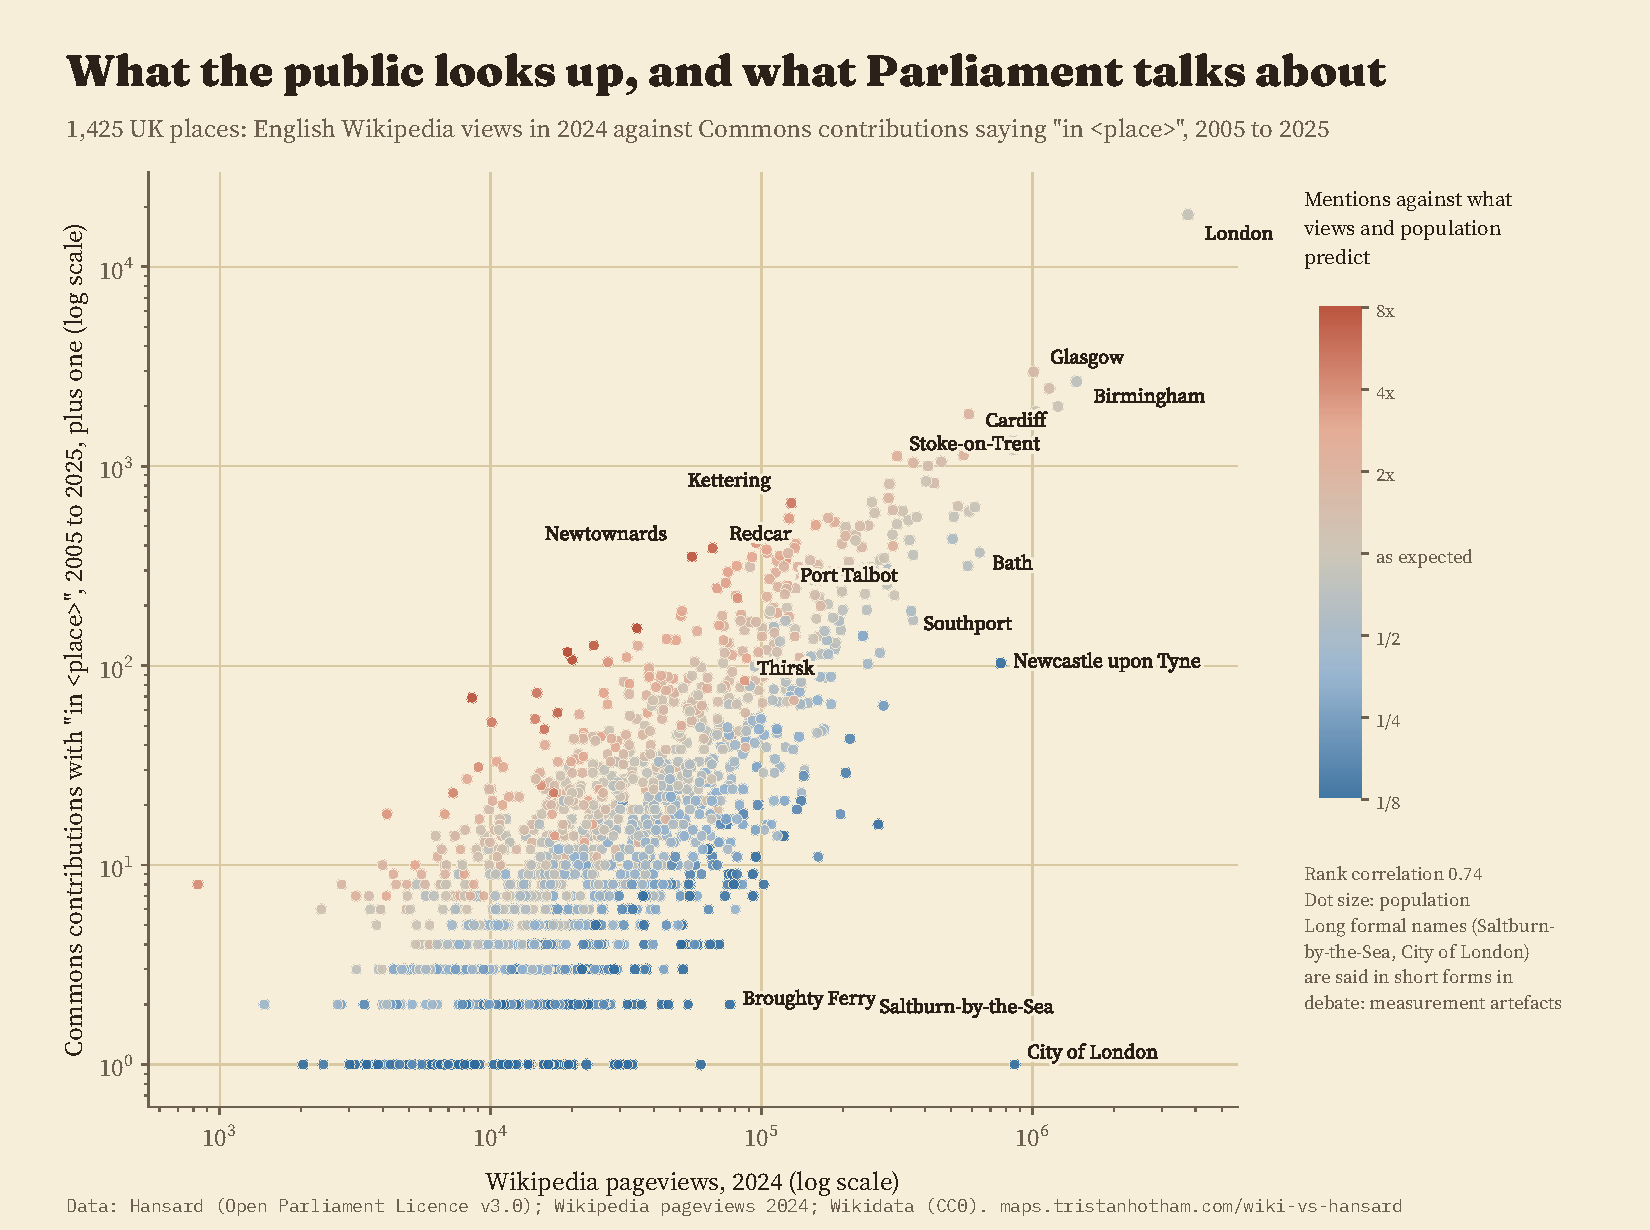
\includegraphics[width=\textwidth]{f_scatter.pdf}\caption{Wikipedia pageviews in 2024 against Commons contributions containing ``in'' plus the place name, 2005 to 2025, $N$ = 1,425. Colour: mentions relative to the number expected from views and population; size: population. Long formal names at the bottom right are measurement artefacts (Section~\ref{sec:design}).}\label{fig:scatter}\end{figure}

\begin{table}[tbp]\centering\small\caption{Main models of ``in'' mentions, 2005 to 2025. Columns 1 to 3: Poisson pseudo-maximum likelihood; column 4: OLS of $\log(1+Y)$. Standard errors clustered by local authority in parentheses. $^{*}p<.05$, $^{**}p<.01$, $^{***}p<.001$. Region coefficients in Appendix Table~\ref{tab:full}.}\label{tab:main}\begin{tabular}{lcccc}\toprule & M0 & M1 (main) & M1, no distance & OLS\\\midrule
log pageviews 2024 &  & $0.541^{***}$ & $0.536^{***}$ & $0.605^{***}$\\
 &  & (0.043) & (0.043) & (0.035)\\
log population & $1.065^{***}$ & $0.601^{***}$ & $0.621^{***}$ & $0.495^{***}$\\
 & (0.032) & (0.040) & (0.037) & (0.037)\\
Seat-name share & $0.957^{***}$ & $0.794^{***}$ & $0.770^{***}$ & $0.916^{***}$\\
 & (0.083) & (0.078) & (0.072) & (0.069)\\
log(1 + km to London) & $0.016$ & $-0.062$ &  & $0.325^{***}$\\
 & (0.073) & (0.065) &  & (0.083)\\
Deprivation (SD) & $-0.084^{*}$ & $-0.029$ & $-0.044$ & $-0.024$\\
 & (0.036) & (0.031) & (0.030) & (0.031)\\
Qualified title & $-0.136$ & $-0.093$ & $-0.093$ & $0.171^{**}$\\
 & (0.081) & (0.075) & (0.074) & (0.052)\\
\midrule Region fixed effects & yes & yes & yes & yes\\
$N$ & 1,425 & 1,425 & 1,425 & 1,425\\
Clusters (local authorities) & \multicolumn{4}{c}{353}\\
\bottomrule\end{tabular}\end{table}

\subsection{Seat names and parliamentary attention (H2)}
Places whose name was part of a seat name throughout the period receive 121\% more ``in'' mentions than places with the same pageviews, population and region (95\% CI 90 to 158\%), the largest association in the model (Figure~\ref{fig:effects}). Where the seat carries the place's name alone (Kettering, Redcar), the additional association is 49\% (31 to 71\%) over and above the general seat-name share. The permutation test gives a coefficient of 0.79 against a permutation mean of 0.07 (standard deviation 0.07); none of 1,000 draws reached the observed value ($p$ = 0.001). The ``in'' measure excludes the formula ``the hon. Member for''; with the any-mention outcome, which includes it, the seat association rises to 624\%, as it mechanically should.

Two further mechanical channels remain, and a check added at review addresses them (exploratory). First, phrase overlap: Hansard's phrase search counts ``in Bury North'' as ``in Bury'', so a place whose name begins a longer seat name collects some mentions of the seat. Second, referent: where the seat is called just by the place name, ``in Kettering'' may mean the constituency rather than the town. Splitting the seat-name share into three mutually exclusive types (seat names that begin with the place and go on, 211 places; seats called just the place, 186; and names that appear only later in a seat name, such as Morley in Leeds South West and Morley, 155), the associations are 111\% (76 to 155), 133\% (98 to 175) and 67\% (23 to 126). The last type is free of both artefacts, because ``in Leeds South West and Morley'' does not contain ``in Morley'' and nobody calls that seat ``Morley''; its association is smaller but clearly positive. Phrase overlap is therefore not the main source of the seat association, but part of the larger associations for the other two types may reflect it or the constituency referent, which these data cannot separate.

The within-place design gives an association of 109\% (44 to 201\%, 28,224 place-years). But the placebo fails: adding the seat-name status two years ahead, the lead coefficient is 54\% (23 to 93\%) and the contemporaneous coefficient falls to 41\% ($-$2 to 102\%) (Table~\ref{tab:within}). The exploratory event study (Figure~\ref{fig:event}) shows why. The 87 places that first gained a seat name in 2024 had about half their 2023 level of mentions in 2015 (-56\%), rising unevenly to -21\% in 2022, and then rose to 24\% above the 2023 level in 2024 and 58\% in 2025. Boundary commissions name seats after the most prominent places in them, and prominence was rising before the change. The post-change jump is larger than the pre-trend would project, but with only two post-change years, part of 2024 falling before the election, and possible anticipation once the proposals were published, the within-place estimate is best read as an upper bound on the effect of the name, on the assumption that the earlier rise would have continued. For the 2010 change alone (2005 to 2023) the association is 65\% (27 to 115\%) and, with the lead, 26\% ($-$6 to 69\%). Within places, separating changes in seat names that begin with the place from the rest gives similar associations (116\% and 105\%), so the within-place pattern is not a phrase-overlap artefact either. H2 is supported cross-sectionally; whether the name itself causes the attention cannot be established with these data.

\begin{figure}[tbp]\centering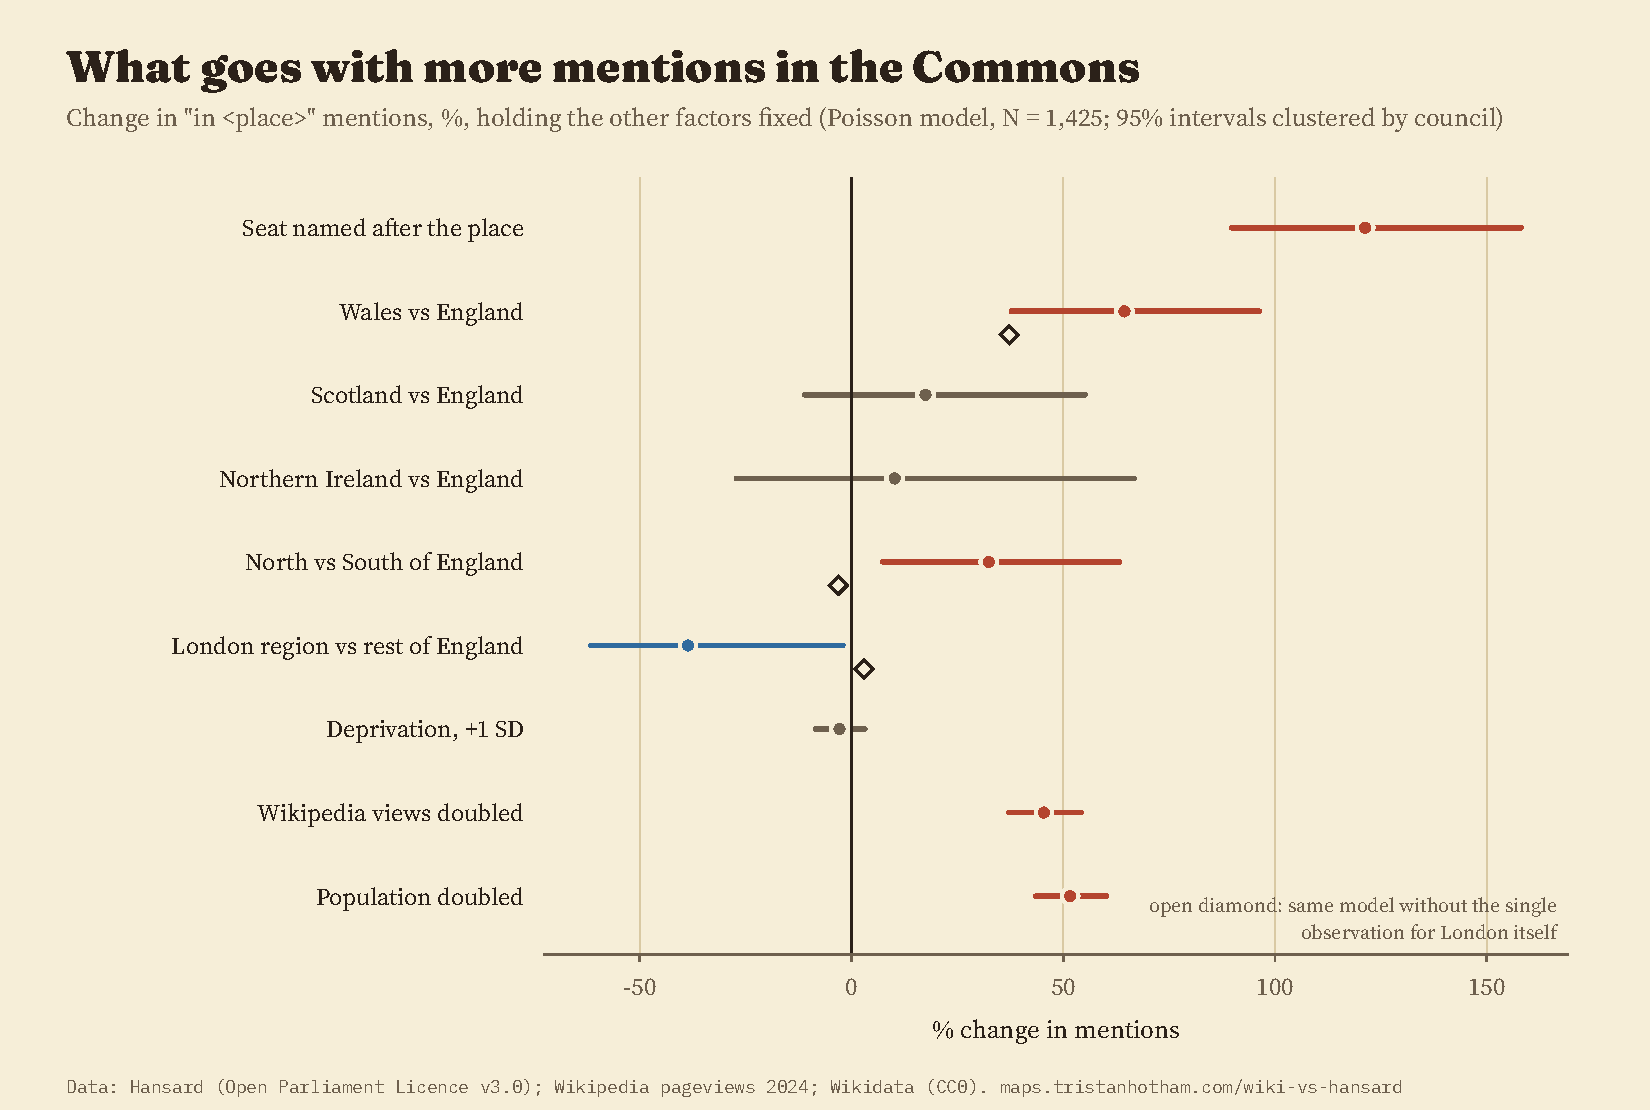
\includegraphics[width=\textwidth]{f_effects.pdf}\caption{Percentage differences in expected ``in'' mentions from M1 with 95\% intervals clustered by local authority ($N$ = 1,425). Diamonds: the same model without the observation for London itself.}\label{fig:effects}\end{figure}

\begin{table}[tbp]\centering\small\caption{Within-place models of yearly ``in'' mentions (PPML, place and year fixed effects, standard errors clustered by local authority). Percentage differences with 95\% intervals.}\label{tab:within}\begin{tabular}{lrrr}\toprule Model & Seat name now & Seat name in two years & Place-years\\\midrule
M2, 2005 to 2025 & 109 [44, 201] & & 28,224\\
M2 with lead (placebo) & 41 [$-$2, 102] & 54 [23, 93] & 28,224\\
Fake timing (lead only) & & 93 [45, 156] & \\
2005 to 2023 (2010 change only) & 65 [27, 115] & & 25,042\\
2005 to 2023 with lead & 26 [$-$6, 69] & 52 [20, 94] & \\
\bottomrule\end{tabular}\end{table}

\begin{figure}[tbp]\centering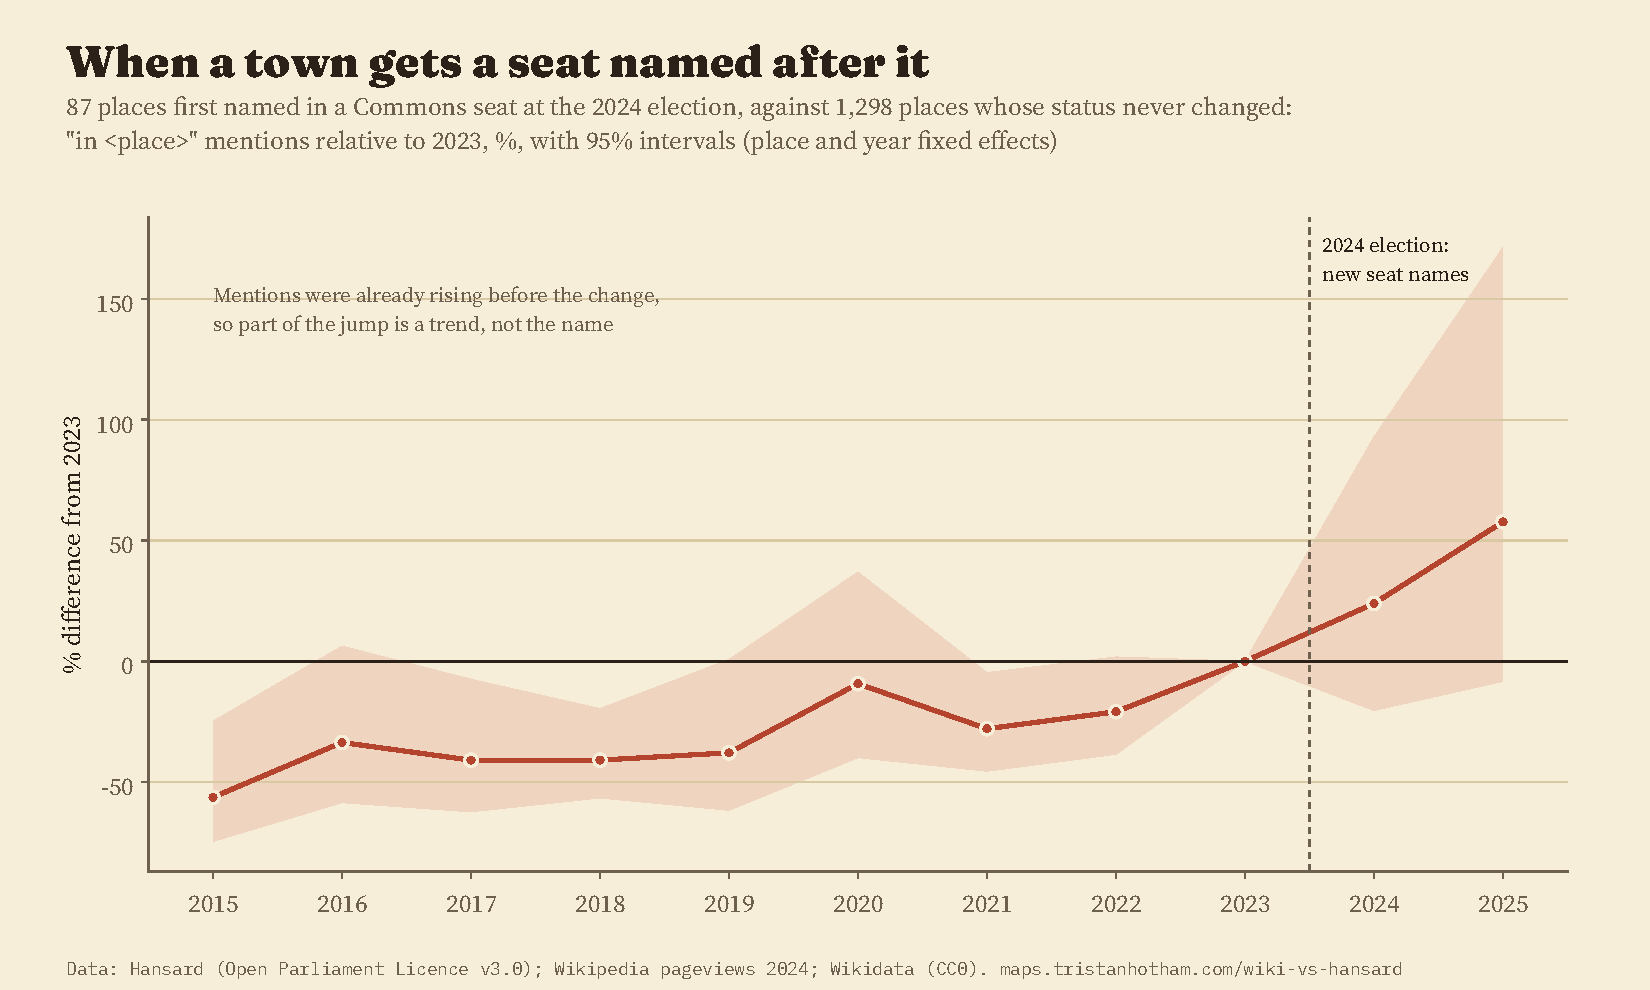
\includegraphics[width=\textwidth]{f_event.pdf}\caption{Event study (exploratory): yearly ``in'' mentions of the 87 places first named in a Commons seat at the 2024 general election, relative to 2023, against 1,298 places whose status did not change, with place and year fixed effects and 95\% intervals clustered by local authority.}\label{fig:event}\end{figure}

\subsection{Nations and regions (H3)}
Contrary to H3a, places in the devolved nations do not receive fewer Commons mentions than English places with the same attention and population. The pooled contrast in M1 is 34\% (10 to 64\%). It is driven by Wales: Welsh places receive 64\% more mentions (38 to 96\%), while the Scottish (17\%, $-$11 to 55) and Northern Irish (10\%, $-$27 to 67) contrasts are imprecise. The Welsh contrast is positive in every robustness check (range 20 to 67\%).

Within England, M1 gives northern places 32\% more mentions than southern places (7 to 63\%), which runs against the voice-deficit view, and places in the London region $-$39\% fewer than the rest of England. These two contrasts, and the pooled devolved contrast, are not robust. Dropping a single observation, London itself, changes them to $-$3\% (north versus south), 3\% (London region) and $-$1\% (devolved nations), all with intervals spanning zero. London has 3,750,408 pageviews and 18,243 mentions; in a Poisson model it carries great weight in the London region effect, and through the distance term and the reference category it moves the other contrasts. Deprivation is unrelated to mentions ($-$2.8\% per standard deviation, $-$8.5 to 3.2), so neither the voice-deficit nor the problem-attention prediction finds support at this level of measurement. Distance from London has no association once region is held constant.

\subsection{Stability over time (H4)}
H4 is not supported by the pre-set criterion. Fitting M1 separately to the two periods, the Spearman correlation of place residuals is 0.47, below 0.6, although the rank correlation of the raw mention counts across the periods is 0.77. The elasticity with respect to 2024 pageviews fell from 0.63 (0.53 to 0.72) in 2005 to 2014 to 0.49 (0.39 to 0.58) in 2015 to 2025; in a stacked model the difference is $-$0.14 ($-$0.23 to $-$0.04). The seat association was similar in both periods (128\% and 117\%; difference in log points $-$0.05, $-$0.21 to 0.11). In an exploratory extension, 2024 pageviews predict mentions in 1945 to 1979 more strongly (elasticity 0.75) than in 1980 to 2004 (0.70), 2005 to 2014 (0.69) or 2015 to 2025 (0.55) (Figure~\ref{fig:time}). Present-day public attention resembles Parliament's older map of Britain more than its current one.

\begin{figure}[tbp]\centering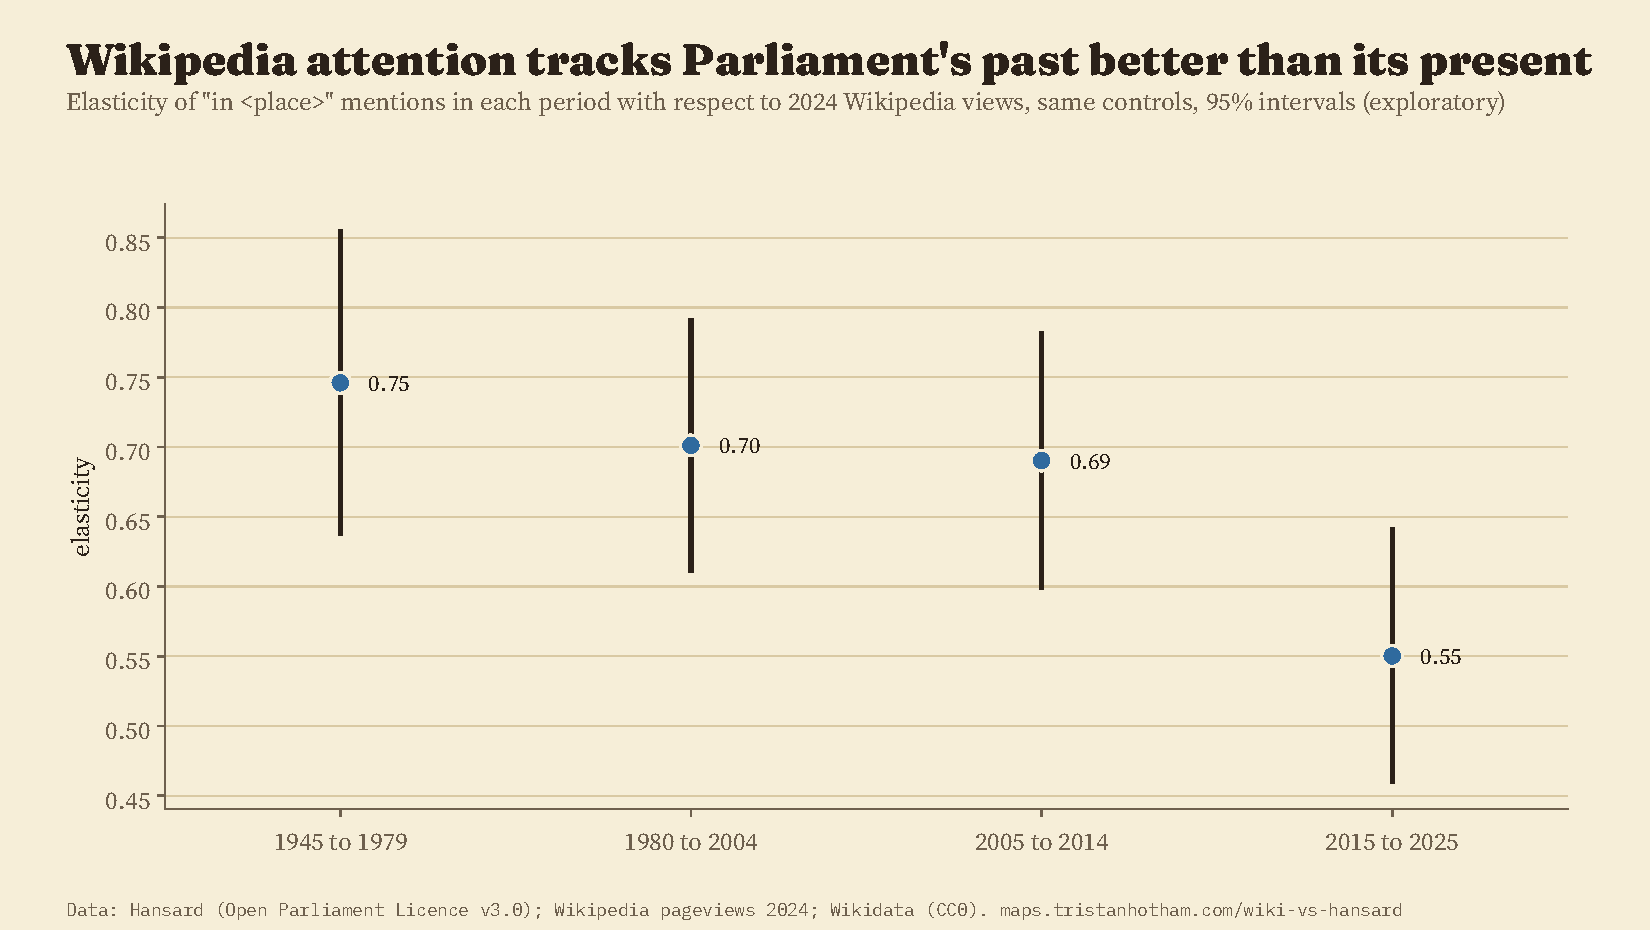
\includegraphics[width=0.92\textwidth]{f_time.pdf}\caption{Elasticity of ``in'' mentions in each period with respect to 2024 pageviews, with the M1 controls except the seat share (exploratory), $N$ = 1,425, 95\% intervals clustered by local authority.}\label{fig:time}\end{figure}

\subsection{Which places diverge}
Among the 674 places expected to receive at least 20 mentions, 57 received at least twice the number expected from their views and population and 220 at most half (Table~\ref{tab:rank}, Figure~\ref{fig:map}). The most over-mentioned are Newtownards (6.9 times), Redcar (5.8), Kettering (4.8) and Dudley (3.6). 84\% of the 25 most over-mentioned places were part of a seat name, against 32\% of the 25 most under-mentioned and 60\% of all ranked places. The under-mentioned are mostly suburbs and secondary towns within seats named after somewhere else (Bamber Bridge, Litherland, Waltham Abbey, Caterham), or named second in a seat (Ewell in Epsom and Ewell, Urmston in Stretford and Urmston) and places whose public prominence is unusually high: Southport, with 357,120 pageviews in a year of national news there, received about half its expected mentions. Large cities sit close to expectation: Edinburgh 1.00, London 0.89, Birmingham 0.77, Glasgow 1.51 and Cardiff 1.87.

\begin{figure}[tbp]\centering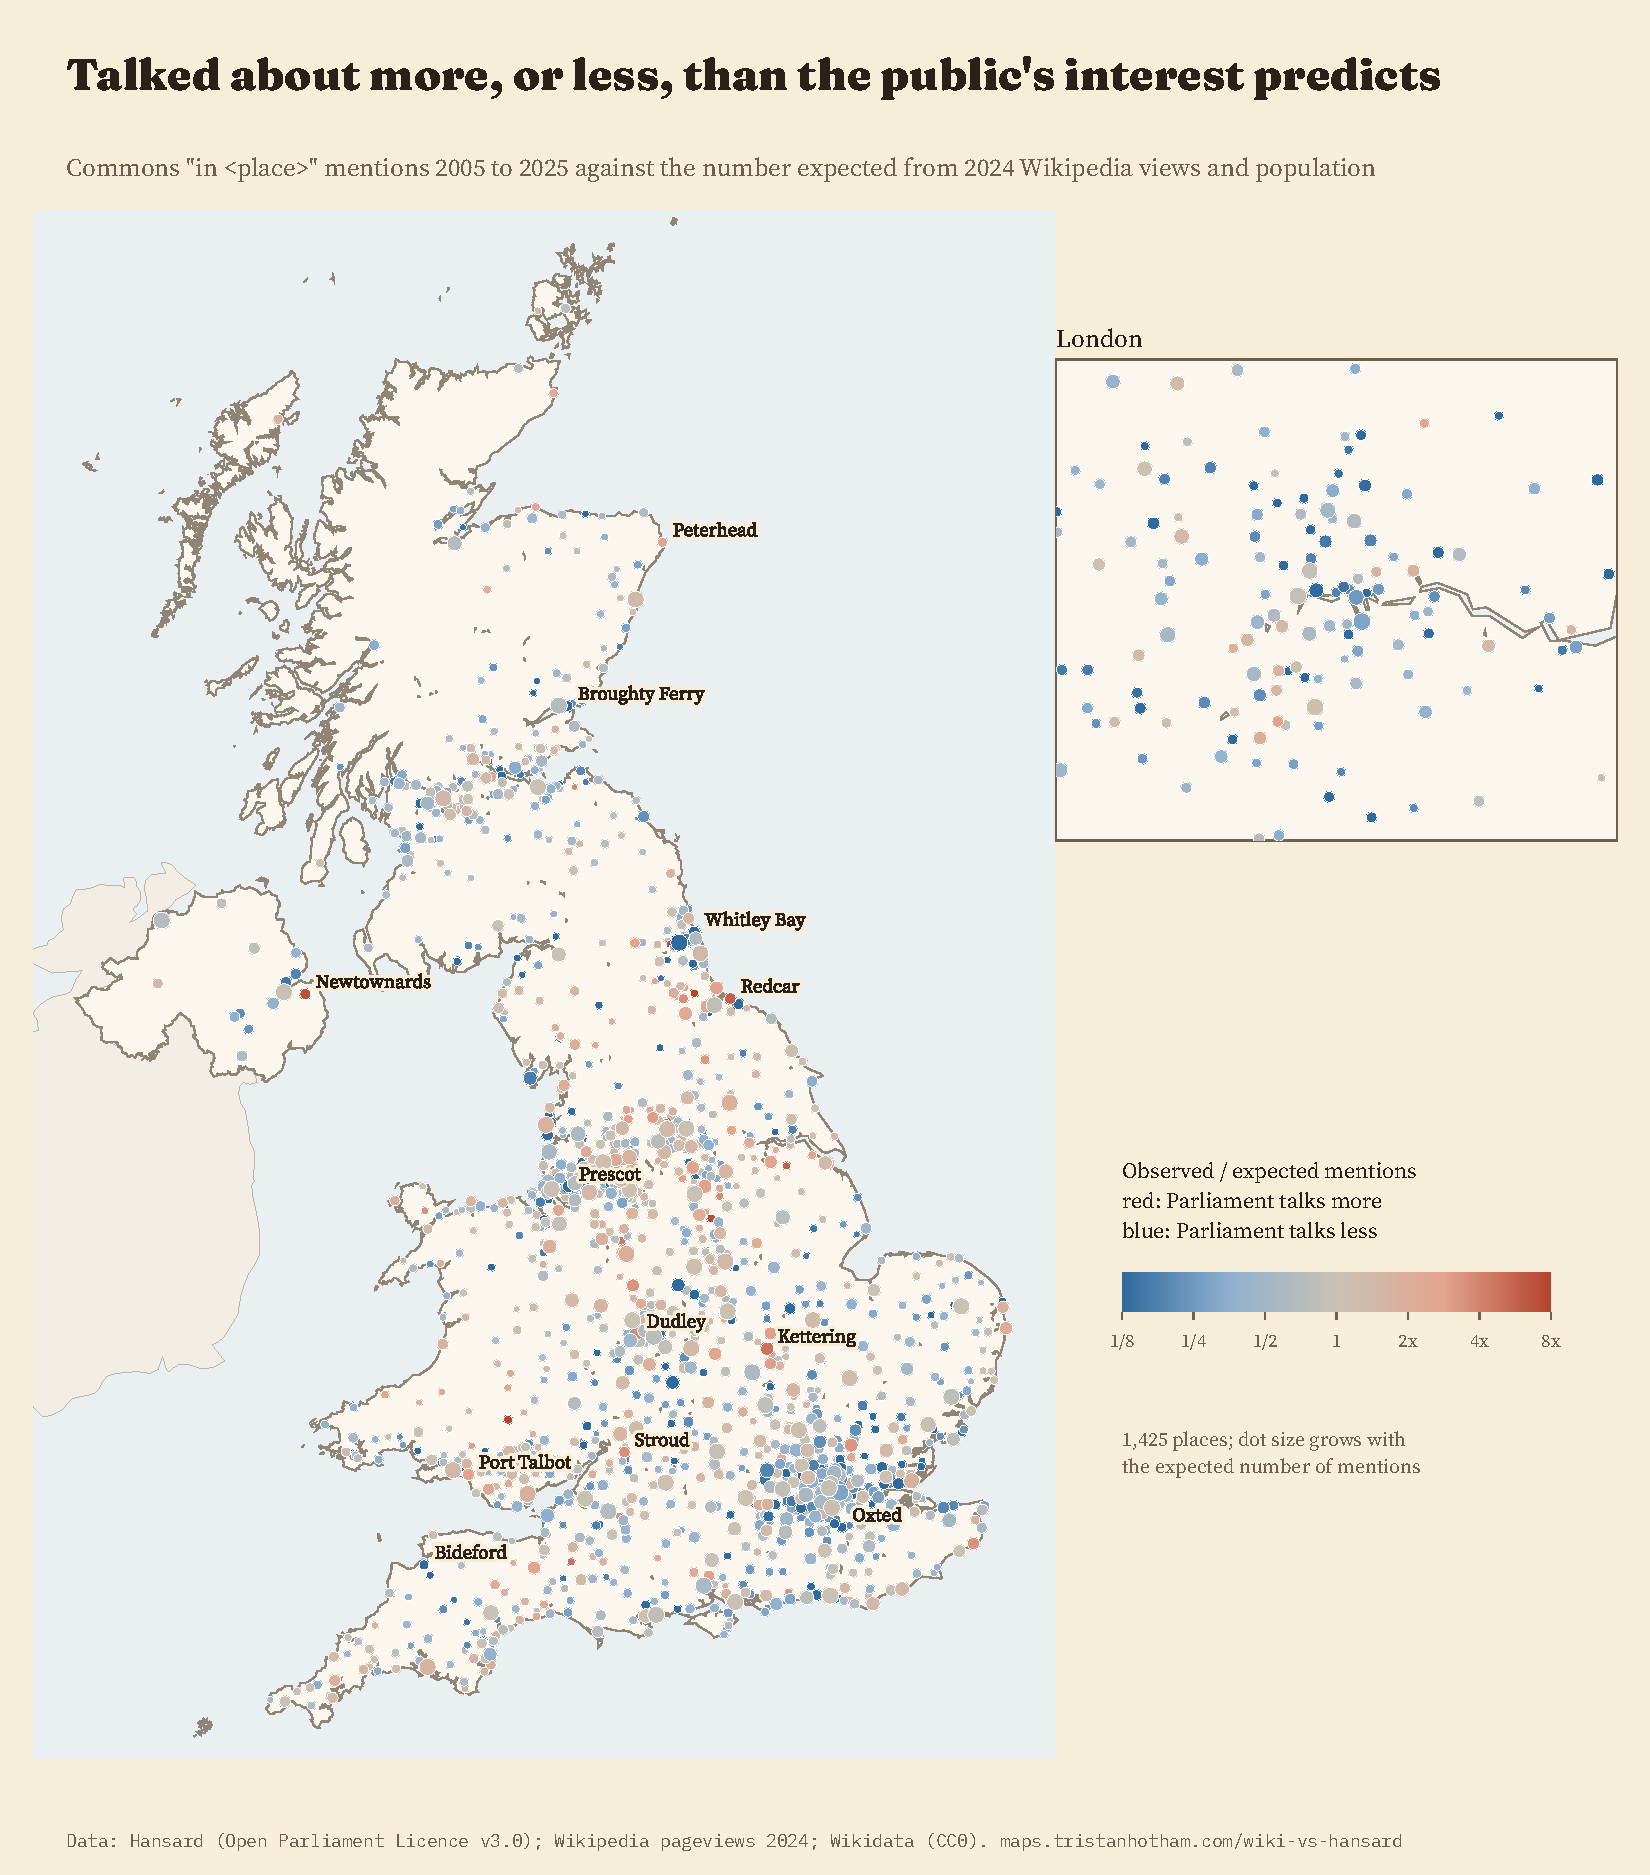
\includegraphics[width=0.86\textwidth]{f_map.pdf}\caption{Observed against expected ``in'' mentions, 2005 to 2025, with expectation from 2024 pageviews and population, $N$ = 1,425. Dot size grows with the expected number of mentions.}\label{fig:map}\end{figure}

\begin{table}[tbp]\centering\footnotesize\caption{The 15 places with the most and fewest ``in'' mentions relative to expectation from 2024 pageviews and population (places expected to receive at least 20 mentions, name-form flagged places excluded). $^\dagger$ part of a seat name in 2005 to 2025.}\label{tab:rank}\setlength{\tabcolsep}{3.5pt}\begin{tabular}{lrrrr@{\hskip 14pt}lrrrr}\toprule \multicolumn{5}{c}{More than expected} & \multicolumn{5}{c}{Less than expected}\\\cmidrule(r){1-5}\cmidrule(l){6-10}Place & Views & Obs. & Exp. & Ratio & Place & Views & Obs. & Exp. & Ratio\\\midrule
Newtownards & 55,381 & 351 & 51 & 6.86 & Becontree & 22,576 & 0 & 52 & 0.01\\
Redcar$^\dagger$ & 65,969 & 387 & 66 & 5.80 & Broughty Ferry$^\dagger$ & 76,446 & 1 & 49 & 0.03\\
Kettering$^\dagger$ & 128,950 & 652 & 137 & 4.76 & Bamber Bridge & 23,144 & 1 & 33 & 0.05\\
Dudley$^\dagger$ & 94,849 & 455 & 126 & 3.62 & Litherland & 42,828 & 1 & 31 & 0.05\\
Newton Aycliffe$^\dagger$ & 27,106 & 103 & 29 & 3.56 & Waltham Abbey & 31,996 & 1 & 28 & 0.05\\
Stroud$^\dagger$ & 81,569 & 217 & 61 & 3.53 & Ewell$^\dagger$ & 20,192 & 1 & 26 & 0.06\\
Dover$^\dagger$ & 123,269 & 340 & 98 & 3.46 & Urmston$^\dagger$ & 28,608 & 2 & 40 & 0.06\\
Stafford$^\dagger$ & 95,538 & 412 & 121 & 3.40 & Chalk Farm & 17,485 & 1 & 21 & 0.07\\
Harlow$^\dagger$ & 126,582 & 546 & 165 & 3.29 & Ascot & 53,394 & 3 & 45 & 0.08\\
Thirsk$^\dagger$ & 86,648 & 83 & 25 & 3.25 & Caterham & 34,087 & 2 & 31 & 0.08\\
Keighley$^\dagger$ & 68,665 & 243 & 79 & 3.08 & Bideford & 37,596 & 2 & 30 & 0.08\\
Wellingborough$^\dagger$ & 73,762 & 259 & 85 & 3.04 & Johnstone & 58,020 & 3 & 38 & 0.09\\
Corby$^\dagger$ & 75,227 & 294 & 98 & 2.99 & Prescot & 92,840 & 8 & 84 & 0.10\\
Rotherham$^\dagger$ & 158,417 & 505 & 170 & 2.96 & Whitley Bay & 79,058 & 7 & 73 & 0.10\\
Eastleigh$^\dagger$ & 50,331 & 177 & 60 & 2.95 & Stamford$^\dagger$ & 92,851 & 6 & 60 & 0.11\\
\bottomrule\end{tabular}\end{table}

\section{Robustness}
Table~\ref{tab:robust} and Figure~\ref{fig:robust} report the pre-specified checks. The pageview elasticity lies between 0.43 and 0.69 in every check that holds population constant; it is lowest when the outcome is restricted to 2024 or 2020 to 2025, the years closest to the pageviews, which suggests the weaker recent link is not an artefact of timing. The seat association lies between 92\% and 154\% (excluding the any-mention outcome, which includes the ``Member for'' formula). The OLS model of $\log(1+Y)$, which weights places equally rather than by their counts, gives an elasticity of 0.60 and a seat association of about 92\%. Leaving out one region at a time, the elasticity ranges from 0.51 to 0.58 and the seat association from 111 to 142\% (Appendix Table~\ref{tab:loro}). The devolved-nation contrast, by contrast, ranges from $-$18 to 39\% across checks and the north/south contrast from $-$14 to 43\%: both depend on the treatment of London and the largest places, as described above, while the Welsh contrast never falls below 20\%. Matching choices make little difference: strict and permissive collision rules, exact titles only, keeping suspect titles and dropping the word-scaled names all leave the main estimates within a few points of M1. Excluding the name-form flagged places raises the elasticity slightly, to 0.59.

\begin{figure}[tbp]\centering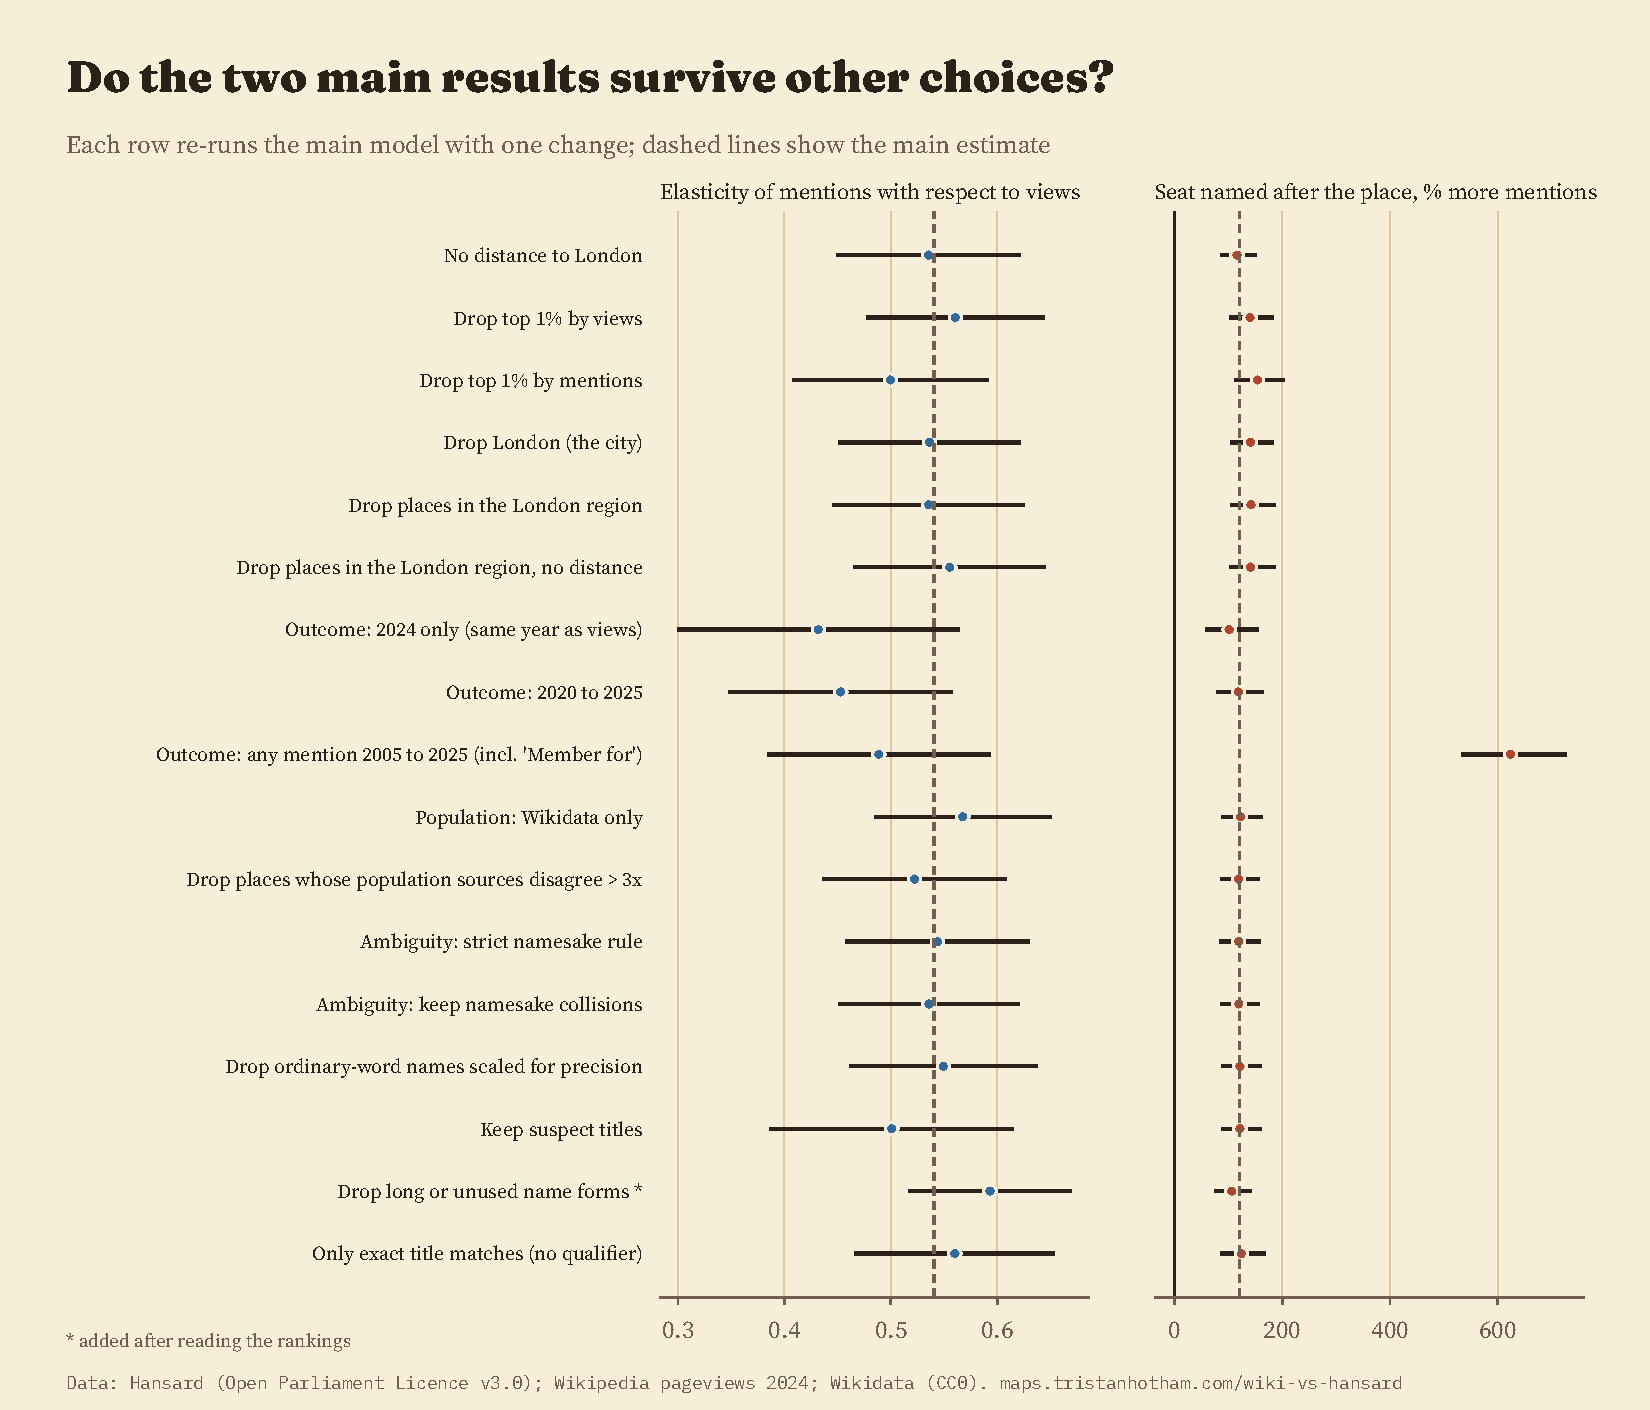
\includegraphics[width=\textwidth]{f_robust.pdf}\caption{The pageview elasticity and the seat association under each robustness check, with 95\% intervals; dashed lines mark M1.}\label{fig:robust}\end{figure}

\begin{table}[tbp]\centering\scriptsize\caption{Robustness checks. Elasticity with respect to pageviews; seat-name, Wales, devolved-nation and north versus south contrasts as percentage differences, 95\% intervals in brackets. The OLS row reports $\exp(b)-1$ of the log-scale coefficients.}\label{tab:robust}\setlength{\tabcolsep}{3pt}\begin{tabular}{p{5.3cm}rlllll}\toprule Check & $N$ & Views & Seat name & Wales & Devolved & North/South\\\midrule
\multicolumn{7}{l}{\textit{R1 specification}}\\
\quad OLS of log(1 + mentions) & 1,425 & 0.60 [0.54, 0.67] & 92 [78, 105] & 23 [$-$4, 58] & $-$16 [$-$32, 4] & $-$14 [$-$33, 10]\\
\quad PPML, views and population only & 1,425 & 0.69 [0.60, 0.78] &  &  &  & \\
\quad PPML, views only & 1,425 & 1.37 [1.26, 1.47] &  &  &  & \\
\quad No distance to London & 1,425 & 0.54 [0.45, 0.62] & 116 [88, 149] & 59 [36, 86] & 25 [8, 45] & 25 [6, 48]\\
\multicolumn{7}{l}{\textit{R3 outliers}}\\
\quad Drop top 1\% by views & 1,410 & 0.56 [0.48, 0.64] & 140 [105, 181] & 20 [$-$4, 51] & $-$18 [$-$36, 4] & $-$2 [$-$23, 25]\\
\quad Drop top 1\% by mentions & 1,410 & 0.50 [0.41, 0.59] & 154 [115, 201] & 24 [$-$1, 56] & $-$14 [$-$32, 10] & $-$4 [$-$25, 24]\\
\quad Drop London (the city) & 1,424 & 0.54 [0.45, 0.62] & 141 [107, 180] & 37 [11, 70] & $-$1 [$-$24, 28] & $-$3 [$-$25, 26]\\
\quad Drop places in the London region & 1,342 & 0.54 [0.45, 0.62] & 142 [106, 184] & 36 [11, 67] & $-$3 [$-$24, 25] & $-$5 [$-$28, 26]\\
\quad Drop places in the London region, no distance & 1,342 & 0.56 [0.47, 0.64] & 141 [105, 184] & 49 [22, 80] & 20 [1, 41] & 20 [2, 42]\\
\multicolumn{7}{l}{\textit{R5 measurement}}\\
\quad Outcome: 2024 only (same year as views) & 1,425 & 0.43 [0.30, 0.56] & 101 [61, 152] & 26 [$-$24, 108] & 23 [$-$9, 66] & 4 [$-$19, 33]\\
\quad Outcome: 2020 to 2025 & 1,425 & 0.45 [0.35, 0.56] & 118 [82, 163] & 36 [6, 76] & 26 [$-$2, 64] & 27 [$-$0, 62]\\
\quad Outcome: any mention 2005 to 2025 (incl. 'Member for') & 1,305 & 0.49 [0.39, 0.59] & 624 [536, 724] & 30 [12, 50] & 22 [4, 44] & 30 [10, 54]\\
\quad Population: Wikidata only & 1,425 & 0.57 [0.49, 0.65] & 123 [90, 161] & 52 [26, 84] & 29 [4, 58] & 23 [$-$1, 54]\\
\quad Drop places whose population sources disagree > 3x & 1,386 & 0.52 [0.44, 0.61] & 119 [88, 155] & 61 [36, 92] & 30 [7, 57] & 29 [5, 58]\\
\quad Ambiguity: strict namesake rule & 1,392 & 0.54 [0.46, 0.63] & 119 [87, 156] & 65 [38, 97] & 35 [10, 65] & 33 [8, 64]\\
\quad Ambiguity: keep namesake collisions & 1,445 & 0.54 [0.45, 0.62] & 119 [88, 155] & 64 [37, 96] & 34 [9, 64] & 32 [7, 62]\\
\quad Drop ordinary-word names scaled for precision & 1,407 & 0.55 [0.46, 0.64] & 121 [90, 159] & 65 [38, 97] & 36 [11, 66] & 34 [8, 65]\\
\quad Keep suspect titles & 1,427 & 0.50 [0.39, 0.61] & 121 [90, 158] & 65 [38, 98] & 36 [11, 66] & 32 [7, 62]\\
\quad Drop long or unused name forms (added after reading the rankings) & 1,322 & 0.59 [0.52, 0.67] & 106 [77, 140] & 61 [36, 90] & 30 [8, 58] & 43 [17, 74]\\
\quad Only exact title matches (no qualifier) & 1,211 & 0.56 [0.47, 0.65] & 124 [89, 166] & 67 [39, 100] & 39 [12, 72] & 34 [7, 67]\\
\midrule\multicolumn{7}{l}{Main model M1: $N$ = 1,425, views 0.54, seat 121 [90, 158], Wales 64 [38, 96]}\\
\multicolumn{7}{l}{Permutation of seat names (1,000 draws): observed 0.794, permutation mean 0.073, sd 0.067, $p$ = 0.001}\\
\bottomrule\end{tabular}\end{table}

\section{Discussion}
\label{sec:discussion}
Three findings stand out. First, parliamentary and public attention to places are closely related but not proportional: the elasticity of about one half means that the places the public finds most interesting are, relative to their prominence, talked about less in the Commons than smaller, less looked-up places. Some of this is what one would expect of a legislature whose members are elected for territories of roughly equal electorate: every seat has an MP with reasons to name its towns, whatever the world's interest in them. Second, the strongest departure from public attention is representational. A place with a seat named after it receives about 2.2 times the mentions of an otherwise similar place. The cross-sectional association is robust and not reproduced by random reassignment, but the within-place evidence shows that places gaining seat names were already rising in prominence. The data are consistent with a causal effect of naming, through MPs' incentives to speak for the places their seat is called after, and with boundary commissions picking up places whose political salience was growing; they cannot separate the two. Third, there is no evidence of a parliamentary voice deficit for the devolved nations or the North of England, once public attention is taken into account. Wales stands out in the other direction. One possibility is that Welsh affairs retain a larger Westminster footprint than devolution alone would suggest, or that Welsh places attract less English Wikipedia attention per head than English ones (some readers use the Welsh Wikipedia). The study cannot distinguish these.

The results speak to the agenda-setting literature by showing that responsiveness to public attention, measured here at the level of places rather than issues, is partial and has declined. They speak to the literature on territorial representation by showing that the electoral map's names track a large share of the variation in which places Parliament discusses. And they temper claims, common since 2016, that places outside London and the South East are systematically ignored in Westminster's talk: on this measure, northern and Welsh places are mentioned at least as much as their public prominence predicts. Mentions are not resources, however, and nothing here says whether being talked about brings benefits.

\paragraph{Limitations.} The design is observational and the main estimates are correlational. The parliamentary measure counts one phrase, ``in'' plus the name, which samples mentions unevenly: long formal names and names usually preceded by ``the'' are undercounted, and names shared with other places or ordinary words required exclusions and scaling that may leave residual error. Commons debate is not the whole of Parliament: written questions, committees and the Lords are excluded. The public measure is one year of English Wikipedia pageviews, which reflect tourism, television and film, news events such as the 2024 attack in Southport, students and visitors as well as residents, and readers anywhere in the world; pageviews of articles with qualified titles are likely depressed. One year of views is set against twenty-one years of debate, so the analysis cannot say whether parliamentary talk leads or follows public interest. The association can run both ways and both measures respond to common shocks: a disaster, a closure or a by-election brings a place into the news, which raises pageviews and Commons mentions together (Southport and Port Talbot in 2024 are examples), and debate may itself send readers to Wikipedia. The pageview elasticity is therefore a description of how the two attentions co-vary, not the effect of one on the other. The exploratory finding that 2024 views track older debates at least as closely as recent ones suggests that pageviews mostly capture long-run cultural prominence rather than recent parliamentary talk, but it does not rule out short-run feedback, which would need monthly pageviews and mentions over several years. Pageviews were collected only for settlements with a Wikidata population of 1,500 or more, so small places and many London districts are absent. Populations mix 2021 Census built-up areas with Wikidata figures of uneven quality. The deprivation measure is at the level of 2010 constituencies and from 2011, and Northern Ireland lacks it. Region contrasts are sensitive to London, which is both the most viewed and the most mentioned place. The seat-name associations combine any effect of representation with the phrase-overlap and constituency-referent channels described in Section~\ref{sec:results}; only the smaller association for names inside longer seat names is free of both. Finally, a place-level analysis says nothing about individual MPs' behaviour or motives.

\section{Conclusion}
Public interest and parliamentary talk about UK places move together, but less than one for one, and the strongest departures from public attention follow the names on the electoral map. There is no sign that the devolved nations or the North of England are spoken of less than their public prominence warrants, and the two kinds of attention drifted apart over two decades. The linked data, code and analysis plan are released so that others can extend the comparison to other years, other measures of public attention, or other parliaments.

\section*{Data availability}
Data and code: Zenodo DOI https://doi.org/10.5281/zenodo.24092583. The repository includes the matched place table, the match log with every rule applied, the place by year panel, all model coefficients and the scripts that reproduce every number in this paper. An interactive map is at \url{https://maps.tristanhotham.com/wiki-vs-hansard/}.

\section*{AI statement}
I wrote the text, with drafting and editing assistance from Claude (Anthropic), which also helped prepare the analysis code. I reviewed and checked all text and results.

\section*{Licences}
Hansard: Contains Parliamentary information licensed under the Open Parliament Licence v3.0. Wikidata and Wikimedia pageview data: CC0. 2011 Census, ONS boundaries and Census 2021 built-up areas: Open Government Licence v3.0. This paper: CC BY 4.0.

\bibliographystyle{plainnat}
\begin{thebibliography}{99}
\bibitem[Abadie et~al.(2023)]{Abadie2023} Abadie, A., Athey, S., Imbens, G. W. and Wooldridge, J. M. (2023) When should you adjust standard errors for clustering? \emph{Quarterly Journal of Economics} 138(1): 1-35.
\bibitem[Baumgartner and Jones(1993)]{BaumgartnerJones1993} Baumgartner, F. R. and Jones, B. D. (1993) \emph{Agendas and Instability in American Politics}. Chicago: University of Chicago Press.
\bibitem[Bettencourt et~al.(2007)]{Bettencourt2007} Bettencourt, L. M. A., Lobo, J., Helbing, D., K\"uhnert, C. and West, G. B. (2007) Growth, innovation, scaling, and the pace of life in cities. \emph{Proceedings of the National Academy of Sciences} 104(17): 7301-7306. doi:10.1073/pnas.0610172104.
\bibitem[Bevan and Jennings(2014)]{BevanJennings2014} Bevan, S. and Jennings, W. (2014) Representation, agendas and institutions. \emph{European Journal of Political Research} 53(1): 37-56. doi:10.1111/1475-6765.12023.
\bibitem[Bowler(2010)]{Bowler2010} Bowler, S. (2010) Private members' bills in the UK Parliament: is there an `electoral connection'? \emph{Journal of Legislative Studies} 16(4): 476-494. doi:10.1080/13572334.2010.519457.
\bibitem[Cain et~al.(1987)]{CainFerejohnFiorina1987} Cain, B., Ferejohn, J. and Fiorina, M. (1987) \emph{The Personal Vote: Constituency Service and Electoral Independence}. Cambridge, MA: Harvard University Press.
\bibitem[Cameron and Miller(2015)]{CameronMiller2015} Cameron, A. C. and Miller, D. L. (2015) A practitioner's guide to cluster-robust inference. \emph{Journal of Human Resources} 50(2): 317-372.
\bibitem[Correia et~al.(2020)]{Correia2020} Correia, S., Guimar\~aes, P. and Zylkin, T. (2020) Fast Poisson estimation with high-dimensional fixed effects. \emph{Stata Journal} 20(1): 95-115. doi:10.1177/1536867X20909691.
\bibitem[Cramer(2016)]{Cramer2016} Cramer, K. J. (2016) \emph{The Politics of Resentment: Rural Consciousness in Wisconsin and the Rise of Scott Walker}. Chicago: University of Chicago Press.
\bibitem[Eggers and Spirling(2014)]{EggersSpirling2014} Eggers, A. C. and Spirling, A. (2014) Ministerial responsiveness in Westminster systems: institutional choices and House of Commons debate, 1832-1915. \emph{American Journal of Political Science} 58(4): 873-887. doi:10.1111/ajps.12090.
\bibitem[Eulau and Karps(1977)]{EulauKarps1977} Eulau, H. and Karps, P. D. (1977) The puzzle of representation: specifying components of responsiveness. \emph{Legislative Studies Quarterly} 2(3): 233-254. doi:10.2307/439340.
\bibitem[Fernandes et~al.(2018)]{Fernandes2018} Fernandes, J. M., Leston-Bandeira, C. and Schwemmer, C. (2018) Election proximity and representation focus in party-constrained environments. \emph{Party Politics} 24(6): 674-685. doi:10.1177/1354068817689955.
\bibitem[Galtung and Ruge(1965)]{GaltungRuge1965} Galtung, J. and Ruge, M. H. (1965) The structure of foreign news: the presentation of the Congo, Cuba and Cyprus crises in four Norwegian newspapers. \emph{Journal of Peace Research} 2(1): 64-91.
\bibitem[Garc\'ia-Gavilanes et~al.(2017)]{GarciaGavilanes2017} Garc\'ia-Gavilanes, R., Mollgaard, A., Tsvetkova, M. and Yasseri, T. (2017) The memory remains: understanding collective memory in the digital age. \emph{Science Advances} 3(4): e1602368. doi:10.1126/sciadv.1602368.
\bibitem[Generous et~al.(2014)]{Generous2014} Generous, N., Fairchild, G., Deshpande, A., Del Valle, S. Y. and Priedhorsky, R. (2014) Global disease monitoring and forecasting with Wikipedia. \emph{PLoS Computational Biology} 10(11): e1003892. doi:10.1371/journal.pcbi.1003892.
\bibitem[Ginsberg et~al.(2009)]{Ginsberg2009} Ginsberg, J., Mohebbi, M. H., Patel, R. S., Brammer, L., Smolinski, M. S. and Brilliant, L. (2009) Detecting influenza epidemics using search engine query data. \emph{Nature} 457(7232): 1012-1014. doi:10.1038/nature07634.
\bibitem[Graham et~al.(2014)]{Graham2014} Graham, M., Hogan, B., Straumann, R. K. and Medhat, A. (2014) Uneven geographies of user-generated information: patterns of increasing informational poverty. \emph{Annals of the Association of American Geographers} 104(4): 746-764.
\bibitem[Hotham(2026a)]{Hotham2026} Hotham, T. (2026a) Mentioned in the House: which places does Parliament talk about? Place mentions in House of Commons debates, 1909 to 2026. Zenodo. doi:10.5281/zenodo.23761431.
\bibitem[Hotham(2026b)]{Hotham2026b} Hotham, T. (2026b) Who Won Here? Every UK general election since 1832 on one map. Zenodo. doi:10.5281/zenodo.23761425.
\bibitem[Jennings and John(2009)]{JenningsJohn2009} Jennings, W. and John, P. (2009) The dynamics of political attention: public opinion and the Queen's Speech in the United Kingdom. \emph{American Journal of Political Science} 53(4): 838-854.
\bibitem[Jennings and Stoker(2016)]{JenningsStoker2016} Jennings, W. and Stoker, G. (2016) The bifurcation of politics: two Englands. \emph{Political Quarterly} 87(3): 372-382. doi:10.1111/1467-923X.12228.
\bibitem[Jones and Baumgartner(2005)]{JonesBaumgartner2005} Jones, B. D. and Baumgartner, F. R. (2005) \emph{The Politics of Attention: How Government Prioritizes Problems}. Chicago: University of Chicago Press.
\bibitem[Kellermann(2013)]{Kellermann2013} Kellermann, M. (2013) Sponsoring early day motions in the British House of Commons as a response to electoral vulnerability. \emph{Political Science Research and Methods} 1(2): 263-280. doi:10.1017/psrm.2013.19.
\bibitem[Kellermann(2016)]{Kellermann2016} Kellermann, M. (2016) Electoral vulnerability, constituency focus, and parliamentary questions in the House of Commons. \emph{British Journal of Politics and International Relations} 18(1): 90-106. doi:10.1111/1467-856X.12075.
\bibitem[Kenny(2014)]{Kenny2014} Kenny, M. (2014) \emph{The Politics of English Nationhood}. Oxford: Oxford University Press.
\bibitem[Khadivi and Ramakrishnan(2016)]{Khadivi2016} Khadivi, P. and Ramakrishnan, N. (2016) Wikipedia in the tourism industry: forecasting demand and modeling usage behavior. \emph{Proceedings of the AAAI Conference on Artificial Intelligence} 30(2): 4016-4021. doi:10.1609/aaai.v30i2.19078.
\bibitem[Lemmerich et~al.(2019)]{Lemmerich2019} Lemmerich, F., S\'aez-Trumper, D., West, R. and Zia, L. (2019) Why the world reads Wikipedia: beyond English speakers. In \emph{Proceedings of the Twelfth ACM International Conference on Web Search and Data Mining (WSDM 2019)}, 618-626. doi:10.1145/3289600.3291021.
\bibitem[Mansbridge(2003)]{Mansbridge2003} Mansbridge, J. (2003) Rethinking representation. \emph{American Political Science Review} 97(4): 515-528.
\bibitem[Martin(2011)]{Martin2011} Martin, S. (2011) Using parliamentary questions to measure constituency focus: an application to the Irish case. \emph{Political Studies} 59(2): 472-488. doi:10.1111/j.1467-9248.2011.00885.x.
\bibitem[McCann(2020)]{McCann2020} McCann, P. (2020) Perceptions of regional inequality and the geography of discontent: insights from the UK. \emph{Regional Studies} 54(2): 256-267. doi:10.1080/00343404.2019.1619928.
\bibitem[Mellon(2013)]{Mellon2013} Mellon, J. (2013) Where and when can we use Google Trends to measure issue salience? \emph{PS: Political Science and Politics} 46(2): 280-290. doi:10.1017/S1049096513000279.
\bibitem[Mesty\'an et~al.(2013)]{Mestyan2013} Mesty\'an, M., Yasseri, T. and Kert\'esz, J. (2013) Early prediction of movie box office success based on Wikipedia activity big data. \emph{PLoS ONE} 8(8): e71226. doi:10.1371/journal.pone.0071226.
\bibitem[Moat et~al.(2013)]{Moat2013} Moat, H. S., Curme, C., Avakian, A., Kenett, D. Y., Stanley, H. E. and Preis, T. (2013) Quantifying Wikipedia usage patterns before stock market moves. \emph{Scientific Reports} 3: 1801.
\bibitem[Norton and Wood(1993)]{NortonWood1993} Norton, P. and Wood, D. M. (1993) \emph{Back from Westminster: British Members of Parliament and Their Constituents}. Lexington: University Press of Kentucky.
\bibitem[Pitkin(1967)]{Pitkin1967} Pitkin, H. F. (1967) \emph{The Concept of Representation}. Berkeley: University of California Press.
\bibitem[Proksch and Slapin(2015)]{ProkschSlapin2015} Proksch, S.-O. and Slapin, J. B. (2015) \emph{The Politics of Parliamentary Debate: Parties, Rebels and Representation}. Cambridge: Cambridge University Press.
\bibitem[Rodr\'iguez-Pose(2018)]{RodriguezPose2018} Rodr\'iguez-Pose, A. (2018) The revenge of the places that don't matter (and what to do about it). \emph{Cambridge Journal of Regions, Economy and Society} 11(1): 189-209.
\bibitem[Russo(2011)]{Russo2011} Russo, F. (2011) The constituency as a focus of representation: studying the Italian case through the analysis of parliamentary questions. \emph{Journal of Legislative Studies} 17(3): 290-301. doi:10.1080/13572334.2011.595122.
\bibitem[Santos Silva and Tenreyro(2006)]{SantosSilvaTenreyro2006} Santos Silva, J. M. C. and Tenreyro, S. (2006) The log of gravity. \emph{Review of Economics and Statistics} 88(4): 641-658.
\bibitem[Searing(1994)]{Searing1994} Searing, D. D. (1994) \emph{Westminster's World: Understanding Political Roles}. Cambridge, MA: Harvard University Press.
\bibitem[Singer et~al.(2017)]{Singer2017} Singer, P., Lemmerich, F., West, R., Zia, L., Wulczyn, E., Strohmaier, M. and Leskovec, J. (2017) Why we read Wikipedia. In \emph{Proceedings of the 26th International Conference on World Wide Web (WWW 2017)}, 1591-1600. doi:10.1145/3038912.3052716.
\bibitem[Soroka and Wlezien(2010)]{SorokaWlezien2010} Soroka, S. N. and Wlezien, C. (2010) \emph{Degrees of Democracy: Politics, Public Opinion, and Policy}. Cambridge: Cambridge University Press.
\bibitem[Vivyan and Wagner(2016)]{VivyanWagner2016} Vivyan, N. and Wagner, M. (2016) House or home? Constituent preferences over legislator effort allocation. \emph{European Journal of Political Research} 55(1): 81-99. doi:10.1111/1475-6765.12119.
\bibitem[Vliegenthart and Walgrave(2011)]{VliegenthartWalgrave2011} Vliegenthart, R. and Walgrave, S. (2011) Content matters: the dynamics of parliamentary questioning in Belgium and Denmark. \emph{Comparative Political Studies} 44(8): 1031-1059. doi:10.1177/0010414011405168.
\bibitem[Vrande\v{c}i\'c and Kr\"otzsch(2014)]{Vrandecic2014} Vrande\v{c}i\'c, D. and Kr\"otzsch, M. (2014) Wikidata: a free collaborative knowledgebase. \emph{Communications of the ACM} 57(10): 78-85. doi:10.1145/2629489.
\bibitem[Yasseri and Bright(2016)]{YasseriBright2016} Yasseri, T. and Bright, J. (2016) Wikipedia traffic data and electoral prediction: towards theoretically informed models. \emph{EPJ Data Science} 5: 22. doi:10.1140/epjds/s13688-016-0083-3.
\bibitem[Zittel et~al.(2019)]{Zittel2019} Zittel, T., Nyhuis, D. and Baumann, M. (2019) Geographic representation in party-dominated legislatures: a quantitative text analysis of parliamentary questions in the German Bundestag. \emph{Legislative Studies Quarterly} 44(4): 681-711. doi:10.1111/lsq.12238.
\end{thebibliography}

\appendix
\section{Full regression tables}
\begin{table}[tbp]\centering\small\caption{M1 in full (PPML; reference region South East; standard errors clustered by local authority).}\label{tab:full}\begin{tabular}{lrrr}\toprule Term & $b$ & SE & $p$\\\midrule
Constant & -8.629 & 0.536 & 0.000\\
log pageviews 2024 & 0.541 & 0.043 & 0.000\\
log population & 0.601 & 0.040 & 0.000\\
Seat-name share & 0.794 & 0.078 & 0.000\\
log(1 + km to London) & -0.062 & 0.065 & 0.340\\
Deprivation (SD) & -0.029 & 0.031 & 0.351\\
Qualified title & -0.093 & 0.075 & 0.215\\
Region: East Midlands & 0.407 & 0.196 & 0.038\\
Region: East of England & 0.166 & 0.095 & 0.080\\
Region: London & -0.196 & 0.195 & 0.313\\
Region: North East & 0.389 & 0.301 & 0.197\\
Region: North West & 0.406 & 0.133 & 0.002\\
Region: Northern Ireland & 0.351 & 0.239 & 0.142\\
Region: Scotland & 0.415 & 0.174 & 0.017\\
Region: South West & 0.331 & 0.118 & 0.005\\
Region: Wales & 0.751 & 0.126 & 0.000\\
Region: West Midlands & 0.311 & 0.139 & 0.025\\
Region: Yorkshire and the Humber & 0.517 & 0.142 & 0.000\\
\midrule $N$ & 1,425 & & \\\bottomrule\end{tabular}\end{table}
\begin{table}[tbp]\centering\small\caption{Leave one region out: M1 re-estimated without each region.}\label{tab:loro}\begin{tabular}{lrlll}\toprule Region left out & $N$ & Views & Seat name (\%) & Devolved vs England (\%)\\\midrule
East Midlands & 1,330 & 0.54 [0.46, 0.63] & 117 [87, 153] & 34 [10, 65]\\
East of England & 1,290 & 0.54 [0.45, 0.63] & 125 [93, 162] & 38 [12, 70]\\
London & 1,342 & 0.54 [0.45, 0.62] & 142 [106, 184] & $-$3 [$-$24, 25]\\
North East & 1,364 & 0.58 [0.50, 0.66] & 112 [81, 148] & 29 [6, 56]\\
North West & 1,260 & 0.51 [0.42, 0.61] & 120 [86, 161] & 40 [12, 75]\\
Northern Ireland & 1,411 & 0.55 [0.46, 0.63] & 127 [95, 164] & 35 [11, 66]\\
Scotland & 1,238 & 0.53 [0.44, 0.62] & 136 [100, 177] & 63 [36, 95]\\
South East & 1,243 & 0.54 [0.44, 0.63] & 118 [84, 159] & 33 [8, 64]\\
South West & 1,262 & 0.54 [0.45, 0.63] & 124 [90, 165] & 39 [12, 72]\\
Wales & 1,288 & 0.51 [0.42, 0.60] & 127 [94, 167] & 18 [$-$10, 56]\\
West Midlands & 1,335 & 0.57 [0.49, 0.66] & 111 [79, 149] & 33 [9, 64]\\
Yorkshire and the Humber & 1,312 & 0.52 [0.43, 0.61] & 114 [82, 152] & 35 [9, 66]\\
\bottomrule\end{tabular}\end{table}
\section{Data construction details}
\label{app:data}
\paragraph{Wikidata settlements.} Items classed as human settlements in the United Kingdom with an English Wikipedia sitelink, exported with QLever; title, population (P1082, any vintage) and coordinate location. 81 items fall outside UK local authority districts by more than 3 km and were removed: 4 of these had pageviews (Gibraltar, Cockburn Town, Road Town, and Swansea Bay City Region, a regional partnership rather than a settlement). Two area items (Somerset, Greater London) were also removed.
\paragraph{Pageviews.} Wikimedia pageview API, per article, English Wikipedia, agent ``user'', summed over 1 January to 31 December 2024; requested for the exact Wikidata sitelink title (a value of zero means no views were recorded under that title).
\paragraph{Matching.} Normalisation: Unicode decomposition with accents removed, lower case, ampersand to ``and'', apostrophes removed, all other non-alphanumeric characters to spaces, ``saint'' to ``st''. Candidate titles: the part before the first comma, with a trailing bracketed qualifier removed. Distance rule: 20 km, ignored for the 16 hand aliases. Median match distance 0.31 km, 95th percentile 1.27 km; 1 match beyond 5 km (Portishead, where the Hansard point is misplaced). Name collisions: another UK settlement with the same normalised base name and at least 25\% of the matched article's views (20, e.g. Farnborough, Ripley, Beeston, Kennington). Suspect titles: views below 2\% of the Wikidata population (3).
\paragraph{Seat names.} 946 seat names in use from 2005 to 2026, with first and last dates of members' spans; a seat counts in a boundary period if its span overlaps the period by more than 30 days. Year weights: 2005 to 2009 belong to the first period, 2010 is split at 6 May, 2011 to 2023 to the second, 2024 is split at 4 July, 2025 to the third.
\paragraph{Name forms.} Terms containing a joining word (on, upon, by, under, le, la, de, in, super, next, cum, en), beginning ``City of'', ending in Minster, Regis, Spa, Magna or Parva, containing an apostrophe, or never found after ``in'' from 1909 to 2025: 103 of the matched places. Used only for the rankings and one robustness check.
\end{document}
